%pdflatex abra.tex
% white background
%convert -density 150x150 abra.pdf abra.png
\documentclass[border={2pt 2pt 2pt 2pt}]{standalone}
\usepackage{tikz}
\usetikzlibrary{calc}
\begin{document}

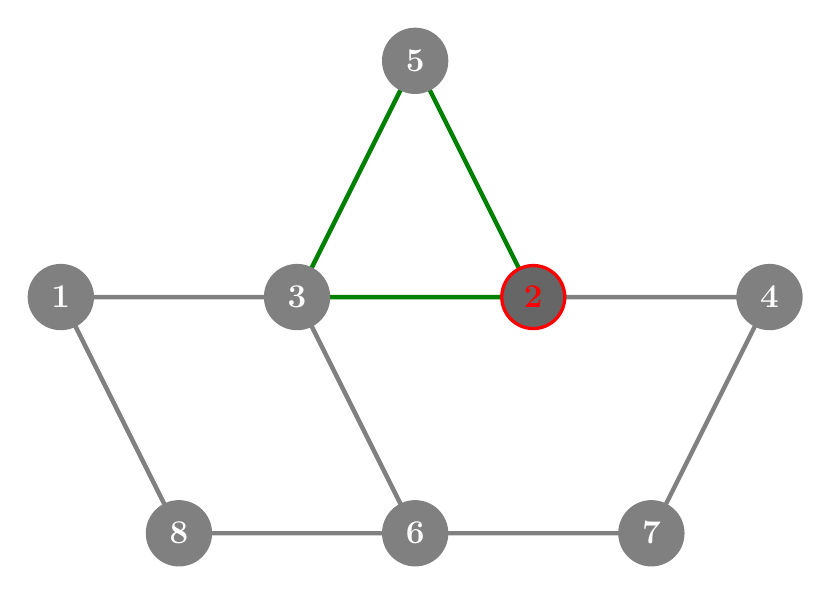
\begin{tikzpicture}
\coordinate (A) at (-3,0);
\coordinate (B) at (3,0);
\coordinate (C) at (0,0);
\coordinate (D) at (6,0);
\coordinate (E) at (1.5,3);
\coordinate (F) at (1.5,-3);
\coordinate (G) at (4.5,-3);
\coordinate (H) at (-1.5,-3);
\draw[gray,ultra thick] (A)--(C)--(F)--(H)--cycle (B)--(D)--(G)--(F);
\draw[green!50!black,ultra thick] (B)--(C)--(E)--cycle;
\draw[gray,very thick,fill=gray] (A) circle [radius=0.4];
\draw[red,very thick,fill=gray!80!black] (B) circle [radius=0.4];
\draw[gray,very thick,fill=gray] (C) circle [radius=0.4];
\draw[gray,very thick,fill=gray] (D) circle [radius=0.4];
\draw[gray,very thick,fill=gray] (E) circle [radius=0.4];
\draw[gray,very thick,fill=gray] (F) circle [radius=0.4];
\draw[gray,very thick,fill=gray] (G) circle [radius=0.4];
\draw[gray,very thick,fill=gray] (H) circle [radius=0.4];
\node[white] at (A) {\large\bf 1};
\node[red] at (B) {\large\bf 2};
\node[white] at (C) {\large\bf 3};
\node[white] at (D) {\large\bf 4};
\node[white] at (E) {\large\bf 5};
\node[white] at (F) {\large\bf 6};
\node[white] at (G) {\large\bf 7};
\node[white] at (H) {\large\bf 8};
\end{tikzpicture}

\end{document}
